%!TEX root = da-screen.tex

The defining property of fast distributed algorithms is \emph{locality}: if we run a distributed algorithm for $t$ time steps, then nodes can only be aware of information that is available within distance at most $t$ from them. In this chapter we will see why this is the case, and what consequences it has.

\section{Locality}

Locality is easiest to understand through an example. Consider the following network, familiar from the previous section:
\begin{center}
    \includegraphics[page=\PIntroId]{figs.pdf}
\end{center}
Let us focus on node number $15$. Initially, there is only one node in the network that is aware of the existence of such a node\mydash the node itself. Let us highlight the set of nodes that are aware of node $15$ at time {\boldmath $t = 0$}:
\begin{center}
    \includegraphics[page=\PIntroTA]{figs.pdf}
\end{center}
All other nodes are completely unaware of the existence of node number $15$. For example, for all that they know, we might equally well have the following instance, in which we do not have any node with identifier $15$:
\begin{center}
    \includegraphics[page=\PIntroIdX]{figs.pdf}
\end{center}

Now let us consider what happens at time {\boldmath $t = 1$}, after one communication round. In this round, all nodes can exchange messages with their neighbours, simultaneously in parallel. Nodes can send anything that they know to their neighbours. In particular, node $15$ can inform its neighbours about its existence, so after one round, its neighbours $33$ and $20$ may also be aware of it:
\begin{center}
    \includegraphics[page=\PIntroTB]{figs.pdf}
\end{center}
However, the crucial observation is that only these three nodes can be aware of the existence of node $15$. For example, consider node $27$. Before the first round, this node and its neighbours were unaware of node $15$; hence during the first round node $27$ could not learn anything about node $15$ from any of its neighbours.

By a similar reasoning, at time {\boldmath $t = 2$}, after two communication rounds, the set of nodes that may be aware of node $15$ consists precisely of those nodes that are within distance $t = 2$ from it:
\begin{center}
    \includegraphics[page=\PIntroTC]{figs.pdf}
\end{center}
And at time {\boldmath $t = 3$} this information may have propagated up to distance $t = 3$, but not any further:
\begin{center}
    \includegraphics[page=\PIntroTD]{figs.pdf}
\end{center}
Of course the same reasoning holds for any node, and for any information related to the node. For example, at time $t = 3$, precisely these nodes are aware of the existence of node $13$, and precisely these nodes know that node $13$ is a node of degree $1$, i.e., it has got only one neighbour:
\begin{center}
    \includegraphics[page=\PIntroTDB]{figs.pdf}
\end{center}

Naturally, if a node stops after time $t$, whatever output it produces can only depend on what it knows, and as we have seen, a node can only know information that is available at distance $t$. This is the crux of locality in distributed computing: time and distance are interchangeable; in a \emph{fast} algorithm, nodes have to make decisions based on information that is available \emph{near} them.

\section{Simple Consequences of Locality}\label{sec:intro-neg-simple}

Recall from Chapter~\ref{ch:intro-pos} that there are very fast algorithms for $3$-colouring paths. However, a path can be also coloured with $2$ colours:
\begin{center}
    \includegraphics[page=\PIntroColTwo]{figs.pdf}
\end{center}
With some thought, we can also come up with a distributed algorithm that finds a $2$-colouring of a path with $n$ nodes in time $O(n)$. An algorithm that works along these lines should do the trick:
\begin{itemize}
    \item First, the endpoints of the path (i.e., nodes of degree $1$) send their identifiers to their neighbours. Other nodes forward this information until all nodes along the path learn the identifiers of the endpoints. This takes $n-1$ communication rounds.
    \begin{center}
        \includegraphics[page=\PIntroTwoColA]{figs.pdf}
    \end{center}
    \item Now the endpoints know each other's identifiers. We elect the endpoint with the smaller identifier as the \emph{leader}.
    \begin{center}
        \includegraphics[page=\PIntroTwoColB]{figs.pdf}
    \end{center}
    \item Finally, the leader colours itself with colour $1$, sends its colour to its neighbour, and stops. The neighbour responds by picking colour $2$, etc.; after $n-1$ rounds, we have coloured all nodes with alternating colours $1$ and $2$, and all nodes have stopped.
    \begin{center}
        \includegraphics[page=\PIntroColTwo]{figs.pdf}
    \end{center}
\end{itemize}
However, in comparison with the algorithm of Section~\ref{sec:intro-pos-id-fast}, this is very slow. Hence we can ask the following question: is it really necessary to spend $\Omega(n)$ rounds in order to find a $2$-colouring of a path?

To reach a contradiction, suppose that there was a deterministic algorithm $A$ that runs in time $o(n)$. In particular, there is an $n_0$ such that for any $n \ge n_0$, the running time of algorithm $A$ is at most $(n-3)/2$. Pick some integer $k \ge n_0/2$, and consider two paths: path $G$ contains $2k$ nodes, numbered $1,2,\dotsc,2k$, and path $H$ contains $2k+1$ nodes, numbered \[1,2,\dotsc,k,2k+1,k+1,k+2,\dotsc,2k.\] Here is an example for $k = 3$:
\begin{center}
    \includegraphics[page=\PIntroLbTwoA]{figs.pdf}
\end{center}
By assumption, the running time $t$ is at most $k-1$ rounds in both cases. In particular, node number $1$ is only aware of the first $k$ nodes along the path, and it must produce its output based on what it sees. As what it sees is the same in $G$ and $H$, we conclude that node $1$ picks the same colour in both instances:
\begin{center}
    \includegraphics[page=\PIntroLbTwoB]{figs.pdf}
\end{center}
By a similar reasoning, node $2k$ (i.e., the last node of the path) has the same neighbourhood up to distance $t$, and therefore it also has to produces the same output in both cases:
\begin{center}
    \includegraphics[page=\PIntroLbTwoC]{figs.pdf}
\end{center}
However, now we reach a contradiction. In path $H$, in any proper $2$-colouring nodes $1$ and $2k$ have the same colour\mydash for example, both of them are of colour $1$, as shown in the following picture:
\begin{center}
    \includegraphics[page=\PIntroLbTwoD]{figs.pdf}
\end{center}
If algorithm $A$ works correctly, it follows that nodes $1$ and $2k$ must produce the same output in path $H$. However, then it follows that nodes $1$ and $2k$ produces the same output also in $G$, too, but this cannot happen in any proper $2$-colouring of $G$.
\begin{center}
    \includegraphics[page=\PIntroLbTwoE]{figs.pdf}
\end{center}
We conclude that algorithm $A$ fails to find a proper $2$-colouring in at least one of these instances.

In summary, we have shown that there is no deterministic algorithm that finds a $2$-colouring in time $o(n)$, even if the algorithm can use unique identifiers. On the other hand, there is a deterministic algorithm that solves the problem in time $O(n)$; we conclude that the distributed computational complexity of $2$-colouring paths is precisely $\Theta(n)$.

While we have focused on deterministic algorithms here, we can use similar ideas to prove an analogous result for randomised algorithms, too\mydash this is left as an exercise.


\section{Not So Simple Consequences of Locality}\label{sec:intro-neg-logstar}

In the previous section we saw that $2$-colouring paths with distributed algorithms takes $\Theta(n)$ rounds. In Chapter~\ref{ch:intro-pos} we saw that $3$-colouring is possible much faster, at least if the identifiers are not too large in comparison with $n$.

For the sake of concreteness, let us consider the following case:
\begin{itemize}
    \item we have a \emph{directed} path with $n$ nodes, so that each node has at most one successor and at most one predecessor,
    \item the unique identifiers are a permutation of the set $\{1,2,\dotsc,n\}$.
\end{itemize}
In this case the algorithm of Section~\ref{sec:intro-pos-id-fast} finds a $3$-colouring in time $O(\log^* n)$; here $\log^*$ is the iterated logarithm function that we studied in Exercise~\ref{ex:logstar}. We will now show that this is optimal

Now we will show that the fast $3$-colouring algorithm is asymptotically optimal: $3$-colouring cannot be solved in time $o(\log^* n)$. We will show that this holds even in the following setting:
Fix an $n$, and let $A$ be a deterministic distributed algorithm that finds a $3$-colouring in this setting. Let $t$ be the running time of algorithm $A$. We will show that $t = \Omega(\log^* n)$.

FIXME: Linial's lower bound.


\section{Exercises}

\begin{ex}[counting]
    Consider the following problem: counting the number of nodes in a path. That is, we are given a path with some unknown number of nodes. All nodes have to stop and output $n$, the number of nodes in the path.
    \begin{subex}
        \item Design a deterministic distributed algorithm that solves the counting problem in time $O(n)$. You can assume that the nodes have unique identifiers.
        \item Prove that it is not possible to solve this problem in time $o(n)$.
    \end{subex}
\end{ex}

\begin{ex}[known $n$]
    In Section~\ref{sec:intro-neg-simple} we saw that $2$-colouring a path with $n$ nodes takes $\Omega(n)$    rounds. Show that the claim holds even if $n$ is known. That is, all nodes are initially aware of their own identifier and of the exact number of nodes in the path.
\end{ex}

\begin{ex}[randomised algorithms]
    Show that there is no randomised distributed algorithm that finds a $2$-colouring in time $o(n)$ with probability at least $0.9$.
\end{ex}

\begin{ex}[maximal independent sets]
    Recall the definition of a maximal independent set from Exercise~\ref{ex:intro-mis}. Prove that it is not possible to find a maximal independent set with a deterministic algorithm in time $o(\log^* n)$. Show that this holds even if we have unique identifiers from set $\{1,2,\dotsc,n\}$.
\end{ex}

\begin{ex}[large independent sets]
    An independent set is a set of nodes $I$ such that for each node $v \in I$, none of its neighbours are in $I$. Consider a path with $n$ nodes. Assume that we have unique identifiers that are bounded by some polynomial of $n$, that is, there is a constant $c$ such that the unique identifiers are from $\{1,2,\dotsc,n^c\}$.
    \begin{subex}
        \item Show that it is trivial to find some independent set in $O(1)$ time with a deterministic distributed algorithm.
        \item Show that there exists an independent set with at least $n/2$ nodes.
        \item Show that finding an independent set with at least $n/2$ nodes takes $\Theta(n)$ rounds.
        \item Design a deterministic distributed algorithm that finds an independent set with at least $n/10$ nodes in time $O(\log^* n)$, with the help of unique identifiers. You can assume that the identifiers are bounded by a polynomial in $n$.
        \item Design a randomised distributed algorithm that finds an independent set so that the \emph{expected} number of nodes in the output is at least $n/10$ and the running time of the algorithm is $O(1)$.
    \end{subex}
\end{ex}

\begin{exs}[tight bounds]
    Consider the following case: we have a directed path with $n$ nodes, and the unique identifiers are a permutation of $\{1,2,\dotsc,n\}$. We know that $3$-colouring is possible in time $O(\log^* n)$, and this is \emph{asymptotically} tight. However, there is no need to settle for asymptotic bounds; we can work out a precise expression for the optimal running time up to small additive constants:
    \begin{subex}
        \item Find a positive constant $c_1$ such that the following holds for all $n$: it is possible to find a $3$-colouring with a deterministic algorithm in time $\frac{1}{2} \log^*(n) + c_1$.
        \item Find a positive constant $c_2$ such that the following holds for all $n$: it is not possible to find a $3$-colouring with a deterministic algorithm in time $\frac{1}{2} \log^*(n) - c_2$.
    \end{subex}
    \hint{For the upper bound, we need to speed up the fast algorithm by a factor of $2$. To do this, consider the following strategy: after each iteration, reverse the directions of the edges. Then consider two iterations of the algorithm, and observe that the new colour of a node $v$ after \emph{two} iterations only depends on the original colours within distance \emph{one} from node $v$. Hence one communication step is enough to simulate two iterations of colour reduction.}
\end{exs}
